\documentclass[12pt,a4paper]{article}
\usepackage[utf8]{inputenc}
\usepackage[left=2.00cm,right=2.00cm,top=2.00cm,bottom=2.00cm]{geometry}
\usepackage{transparent}
\usepackage{amsmath}                                 % AMS Math Package
\usepackage[utf8]{inputenc}
\usepackage{amsthm}                                  % Theorem Formatting
\usepackage{amssymb}                                 % Math symbols such as \mathbb
\usepackage{graphicx}                                % Allows for eps images
%\usepackage[dvips,a4paper,margin=1in,bottom=1in]{geometry}
\usepackage{tensor}

% Sets margins and page size

\usepackage{amsmath, esint,mathrsfs}
\def\doubleunderline#1{\underline{\underline{#1}}}
\renewcommand{\labelenumi}{(\alph{enumi})}                % Use letters for enumerate

\usepackage{enumerate}
\usepackage{caption}

\newcommand{\gv}[1]{\ensuremath{\mbox{\boldmath$ #1 $}}} 
\newcommand{\uv}[1]{\ensuremath{\mathbf{\hat{#1}}}}       % enhetsvektor
\newcommand{\abs}[1]{\left| #1 \right|}                   % abslouttverdi
\newcommand{\avg}[1]{\left< #1 \right>}                   % gjennomsnitt

\newcommand{\der}[2]{\frac{\text{d} #1}{\text{d} #2}}     % derivert
\newcommand{\dd}[2]{\frac{\text{d}^2 #1}{\text{d}#2^2}}   % dobbelderivert
\newcommand{\pd}[2]{\frac{\partial #1}{\partial #2}}      % partiellderiverte
\newcommand{\pdd}[2]{\frac{\partial^2 #1}{\partial #2^2}} % doble partiellderiverte

% Kvantemekanikk:

\newcommand{\ket}[1]{\left| #1 \right>}                    % for Dirac kets
\newcommand{\bra}[1]{\left< #1 \right|}                    % for Dirac bras
\newcommand{\braket}[2]{\left< #1 \vphantom{#2} \right|
	\left. #2 \vphantom{#1} \right>}                       % for Dirac brackets
\newcommand{\matrixel}[3]{\left< #1 \vphantom{#2#3} \right|
	#2 \left| #3 \vphantom{#1#2} \right>}                  % for Dirac matrix elements

% Vektoranalyse

\newcommand{\grad}[1]{\gv{\nabla} #1}                      % gradient
\let\divsymb=\div                                          % nytt navn til div
\renewcommand{\div}[1]{\gv{\nabla} \cdot \v{#1}}           % divergens
\newcommand{\curl}[1]{\gv{\nabla} \times \v{#1}}           % curl


% div macros

\newcommand{\iu}{\textup{i}} % imaginary unit
\newcommand{\e}{\textup{e}} % exponent
\newcommand{\intd}[1]{\int\text{d}#1}

% document layout

\setlength{\parindent}{0em}
\setlength{\parskip}{1em}
\setlength{\parindent}{0pt}

\usepackage{fancyhdr}
\usepackage{titlesec}

\usepackage{nameref}
\makeatletter
\newcommand*{\currentname}{\@currentlabelname}
\makeatother

\author{Sondre Duna Lundemo}

\usepackage{xcolor}

\newcommand\bluetextit[1]{\textcolor{blue}{\textit{\sffamily#1}}}
\newcommand\bluetextbf[1]{\textcolor{blue}{\textbf{\sffamily#1}}}

\pagestyle{fancy}
\renewcommand{\headrulewidth}{0.5pt}
\fancyhf{}
\rhead{\textit{\fontfamily{cmr}\selectfont Sondre Duna Lundemo}}
\lhead{\textsc{\currentname}}
\cfoot{\textemdash \, \thepage \, \textemdash}

\titleformat*{\section}{\bfseries \Large}
\titleformat*{\subsection}{\bfseries\large}
\titleformat*{\subsubsection}{\bfseries \normalsize}

\usepackage{hyperref}
\hypersetup{colorlinks=true,linkcolor=blue}

\fancypagestyle{titlepage}{
	\fancyhf{}
	\fancyfoot[C]{$\dagger$\href{mailto:sondre@duna.no}{\texttt{sondre@duna.no}}}
	\fancyfootoffset{-4cm}
	\renewcommand{\headrulewidth}{0pt}
	\renewcommand\footrulewidth{0.5pt}
}

% theoremstyles

\theoremstyle{plain}
\newtheorem{thm}{Theorem}
\newtheorem{axiom}{Axiom}

\theoremstyle{definition}

\newtheorem{definition}{Definition}
\newtheorem{lemma}{Lemma}
\newtheorem{cor}{Corollary}
\newtheorem{prop}{Proposition}

\theoremstyle{remark}

\newtheorem{remark}{Remark}
\newtheorem{notation}{Notation}

\usepackage{enumitem}

\def\be{\begin{equation}}
\def\ee{\end{equation}}

\def\bse{\begin{equation*}}
\def\ese{\end{equation*}}

\def\bt{\begin{thm}}
\def\et{\end{thm}}

\def\bl{\begin{lemma}}
\def\el{\end{lemma}}

\def\bc{\begin{cor}}
\def\ec{\end{cor}}

\def\br{\begin{remark}}
\def\er{\end{remark}}

\def\bal{\begin{align}}
	\def\eal{\end{align}}
	
\def\bd{\begin{definition}}
	\def\ed{\end{definition}}

\def\bit{\begin{itemize}}
	\def\eit{\end{itemize}}

\def\bt{\begin{thm}}
	\def\et{\end{thm}}

\let\vaccent=\v % rename builtin command \v{} to \vaccent{}
\renewcommand{\v}[1]{\ensuremath{\mathbf{#1}}} % vektor

%miscellaneous shortcuts

\providecommand{\AA}{\mathbb{A}}
\providecommand{\BB}{\mathbb{B}}
\providecommand{\CC}{\mathbb{C}}
\providecommand{\DD}{\mathbb{D}}
\providecommand{\EE}{\mathbb{E}}
\providecommand{\FF}{\mathbb{F}}
\providecommand{\GG}{\mathbb{G}}
\providecommand{\HH}{\mathbb{H}}
\providecommand{\II}{\mathbb{I}}
\providecommand{\JJ}{\mathbb{J}}
\providecommand{\KK}{\mathbb{K}}
\providecommand{\LL}{\mathbb{L}}
\providecommand{\MM}{\mathbb{M}}
\providecommand{\NN}{\mathbb{N}}
\providecommand{\OO}{\mathbb{O}}
\providecommand{\PP}{\mathbb{P}}
\providecommand{\QQ}{\mathbb{Q}}
\providecommand{\RR}{\mathbb{R}}
\providecommand{\SS}{\mathbb{S}}
\providecommand{\TT}{\mathbb{T}}
\providecommand{\UU}{\mathbb{U}}
\providecommand{\VV}{\mathbb{V}}
\providecommand{\WW}{\mathbb{W}}
\providecommand{\XX}{\mathbb{X}}
\providecommand{\YY}{\mathbb{Y}}
\providecommand{\ZZ}{\mathbb{Z}}

\providecommand{\A}{\mathcal{A}}
\providecommand{\B}{\mathcal{B}}
\providecommand{\C}{\mathcal{C}}
\providecommand{\D}{\mathcal{D}}
\providecommand{\E}{\mathcal{E}}
\providecommand{\F}{\mathcal{F}}
\providecommand{\G}{\mathcal{G}}
\providecommand{\H}{\mathcal{H}}
\providecommand{\I}{\mathcal{I}}
\providecommand{\J}{\mathcal{J}}
\providecommand{\K}{\mathcal{K}}
\providecommand{\L}{\mathcal{L}}
\providecommand{\M}{\mathcal{M}}
\providecommand{\N}{\mathcal{N}}
\providecommand{\CO}{\mathcal{O}}
\providecommand{\P}{\mathcal{P}}
\providecommand{\Q}{\mathcal{Q}}
\providecommand{\R}{\mathcal{R}}
\providecommand{\S}{\mathcal{S}}
\providecommand{\T}{\mathcal{T}}
\providecommand{\U}{\mathcal{U}}
\providecommand{\V}{\mathcal{V}}
\providecommand{\W}{\mathcal{W}}
\providecommand{\X}{\mathcal{X}}
\providecommand{\Y}{\mathcal{Y}}
\providecommand{\Z}{\mathcal{Z}}

\begin{document}
	
\begin{titlepage}
	\begin{center}
	\setlength{\parskip}{0em}
	\thispagestyle{titlepage}
	
	\centering{
		\Huge{\textbf{Event driven simulation of a $2$-dimensional gas}}
	}

	\vspace{4mm}
	
	\large{\textbf{Sondre Duna Lundemo}}$\dagger$
	
	\normalsize{Department of Physics, Norwegian University of Science and Technology, Trondheim Norway \\
	TFY4235 - Computational physics
	}

	(\textit{Last updated on \today})
	\end{center}

	\setlength{\parindent}{2em}An event driven approach is used to simulate a gas of hard discs in two dimensions. The framework built is used to study statistical properties of the gas at and towards equilibrium. The numerical results are compared with well known results from classical statistical mechanics. Towards the end, the formation of a crater from a projectile impact on a bed of particles is studied with the gas system. 
	
	\begin{figure}[h]
		\centering
		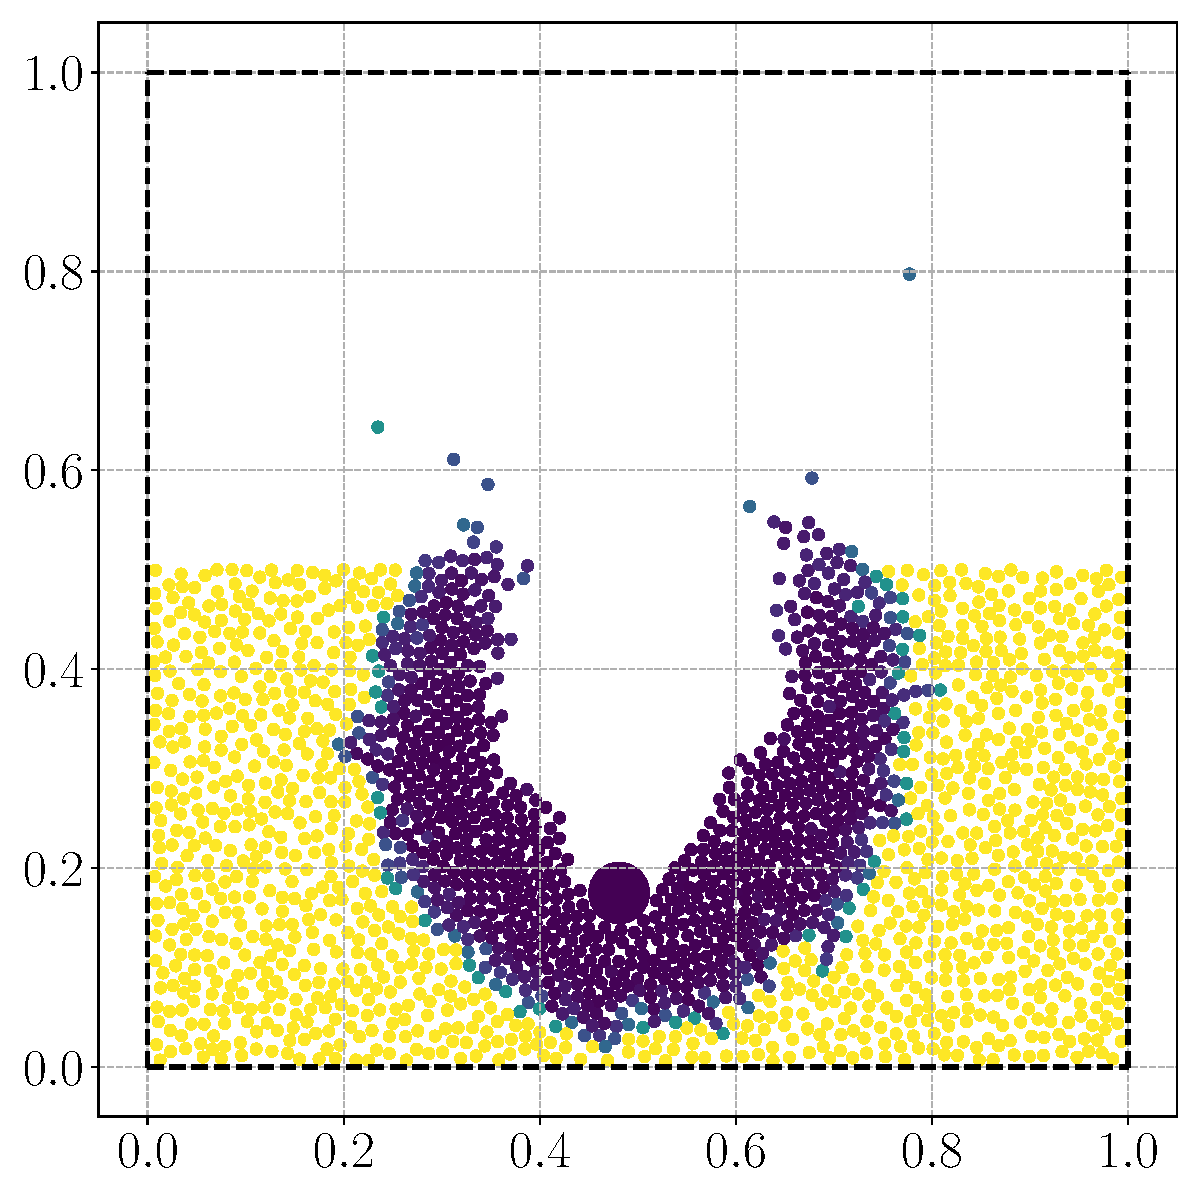
\includegraphics[width=0.7\textwidth]{../fig/crater_2}
	\end{figure}
	

\end{titlepage}

\newpage
\setlength{\parskip}{0em}
\tableofcontents
\setlength{\parskip}{1em}
\newpage

\part{Introduction}
\section{Background}\label{sec:intro}

An event driven approach is used to simulate a gas of hard discs in two dimensions. The framework built is used to study statistical properties of the gas at and towards equilibrium. The numerical results are compared with well known results from classical statistical mechanics. 

The central algorithm for event-driven simulations is the following \cite{event_sim}:

\begin{algorithm}[H]
	Set velocities and positions of all particles in the gas\;
	Choose a stop criterion \;
	\For{each particle in gas}{
		Calculate if and when the particle will collide with all the other particles and the walls \;
		Store all the collision times\;
	}
	\While{not reached stop criterion}{
		Identify the earliest collision \;
		
		\eIf{collision is valid}{
			Move all particles in straight lines until the earliset collision \;
			\For{each particle involved in collision}{
				Calculate if and when the particle will collide with all the other particles and the walls \;
				Store all the collision times\;
			} 
		}{
			discard collsion \;
		}
	}
	\caption{Event driven simulation of a gas.}
\end{algorithm}

In the above algorithm, a collision is \textit{valid} if the particle(s) involved in the collision has \textit{not} collided since the time the collision time was stored. 


\section{Overview of code}\label{sec:overview}

In this section we briefly present how the algorithm is implemented and which considerations are put into the choices of data-structures. The code is written in \texttt{python}.

Although the main algorithm presented in the introduction \ref{sec:intro} invites to a fully object-oriented approach, I have chosen to restrain myself somewhat in that respect. 
The main machinery of the code is collected in a class called \texttt{Gas}, which in essence is a collection of $N$ \texttt{particles} represented their coordinates in phase space, and various methods to manipulate the coordinates of each particle to simulate the gas' time evolution according to the algorithm in section \ref{sec:intro}. 
The most prominent caveat preventing me from doing this is that it might affect the speed of the calculations.
By choosing not to create separate object representing each particle, I found it very simple to move the particles at each time step and also accessing them by ordinary slicing and indexing of arrays. 
Although it is possible to overload operators such that an array of self defined object can be added \textit{like} \texttt{numpy}-arrays, I found this to be impractically slow. 
A quick test of adding the self-made particles compared to simply adding $4\times N$ arrays establishes this observation quite firmly. The listings below shows the time spent on adding two arrays of $50\,000$ particles with each of the mentioned methods.

\begin{lstlisting}
>>>%time particles_array_1 += particles_array_2
CPU times: user 443 us, sys: 101 us, total: 544 us
Wall time: 306 us
\end{lstlisting}

\begin{lstlisting}
>>>%time particles_class_1 += particles_class_2
CPU times: user 34.1 ms, sys: 87 us, total: 34.2 ms
Wall time: 33.2 ms
\end{lstlisting}

The code itself is well documented and should be easy to undestand on its own. However, I would like to point out some solutions that I found to work particularly well. The part of the code that undoubtedly is the most computationally heavy is the one devoted to calculating if and when the particles will collide with all others. The naive approach would be to iterate over each particle and do the calculation for each of them separately. In \texttt{python}, these kind of nested loops will often become impractically slow. I found considerable improvements through vectorising this calculation. 

By essentially replacing the piece of calculation in \ref{lst:loop} by that in \ref{lst:vect} I was able to reduce one of the loops over all of the particles.

\begin{lstlisting}{language=Python,caption= Loop over all particles.,label=lst:loop}
for j in range(self.N):
	delta_x = self.particles[:2,j] - self.particles[:2,i]
	delta_v = self.particles[2:,j] - self.particles[2:,i]
	R_ij    = self.radii[i] + self.radii[j]
	d       = (delta_x @ delta_v)**2 - (delta_v @ delta_v) * ((delta_x @ delta_x) - R_ij**2)
\end{lstlisting}

\begin{lstlisting}{language=Python, caption= Vectorized calculation., label=lst:loop}
mask = np.arange(self.N-1)
mask[i:] += 1

r_ij = self.radii[mask] + self.radii[i]

delta_x = self.particles[:2,mask] - np.reshape(self.particles[:2,i],(2,1))
delta_v = self.particles[2:,mask] - np.reshape(self.particles[2:,i],(2,1))

vv = np.einsum('ij,ij->j',delta_v,delta_v)
vx = np.einsum('ij,ij->j',delta_v,delta_x)
xx = np.einsum('ij,ij->j',delta_x,delta_x)

d = vx ** 2 - vv * ( xx - r_ij**2 )
\end{lstlisting}
\newpage
\part{Results and discussion}

In the following sections, I will present the results from the simulations in the problems. For a more detailed description of the problems consult the exercise sheet \cite{sheet}.

\section{Speed distribution at equilibrium}\label{sec:eq}

The first test is devoted to investigating the distribution of the velocities of the particles after sufficiently long time. From statistical mechanics, we know that the velocities of a $2$-dimensional gas at equilibrium will distribute according to Maxwell's velocity distribution: 
\begin{equation}\label{eq:maxwell}
	p(v) = \frac{mv}{k_B T} \exp{\left(- \frac{mv^2}{2 k_B T}\right)},
\end{equation}
where $k_B$ is Boltzmann's constant, $T$ the absolute temperature, and $m$ the mass of the particles. It is evident that the particles will have to have the same mass for comparing with the known distribution in equation \ref{eq:maxwell}. The case of dissimilar masses is considered in section \ref{sec:mix1} and \ref{sec:mix2}.

We initialise an system of particles with velocities $\mathbf{v} = [v_0 \cos{\theta} , v_0 \sin{\theta}]$ with $\theta \sim \U[0,2\pi]$. The initial distribution of the velocities is therefore $C\delta (v - v_0)$. After simulating the system until equilibrium is reached, i.e. the the average number of particle collision is $\gg 1$, the distribution is as shown in figure \ref{fig:dist_1}. For this simulation, the stop criterion used was that the average number of collisions surpassed $50$. Judging from the plot, it seems to be sufficient for equilibrium to be reached. 

\begin{figure}[htb]
	\centering
	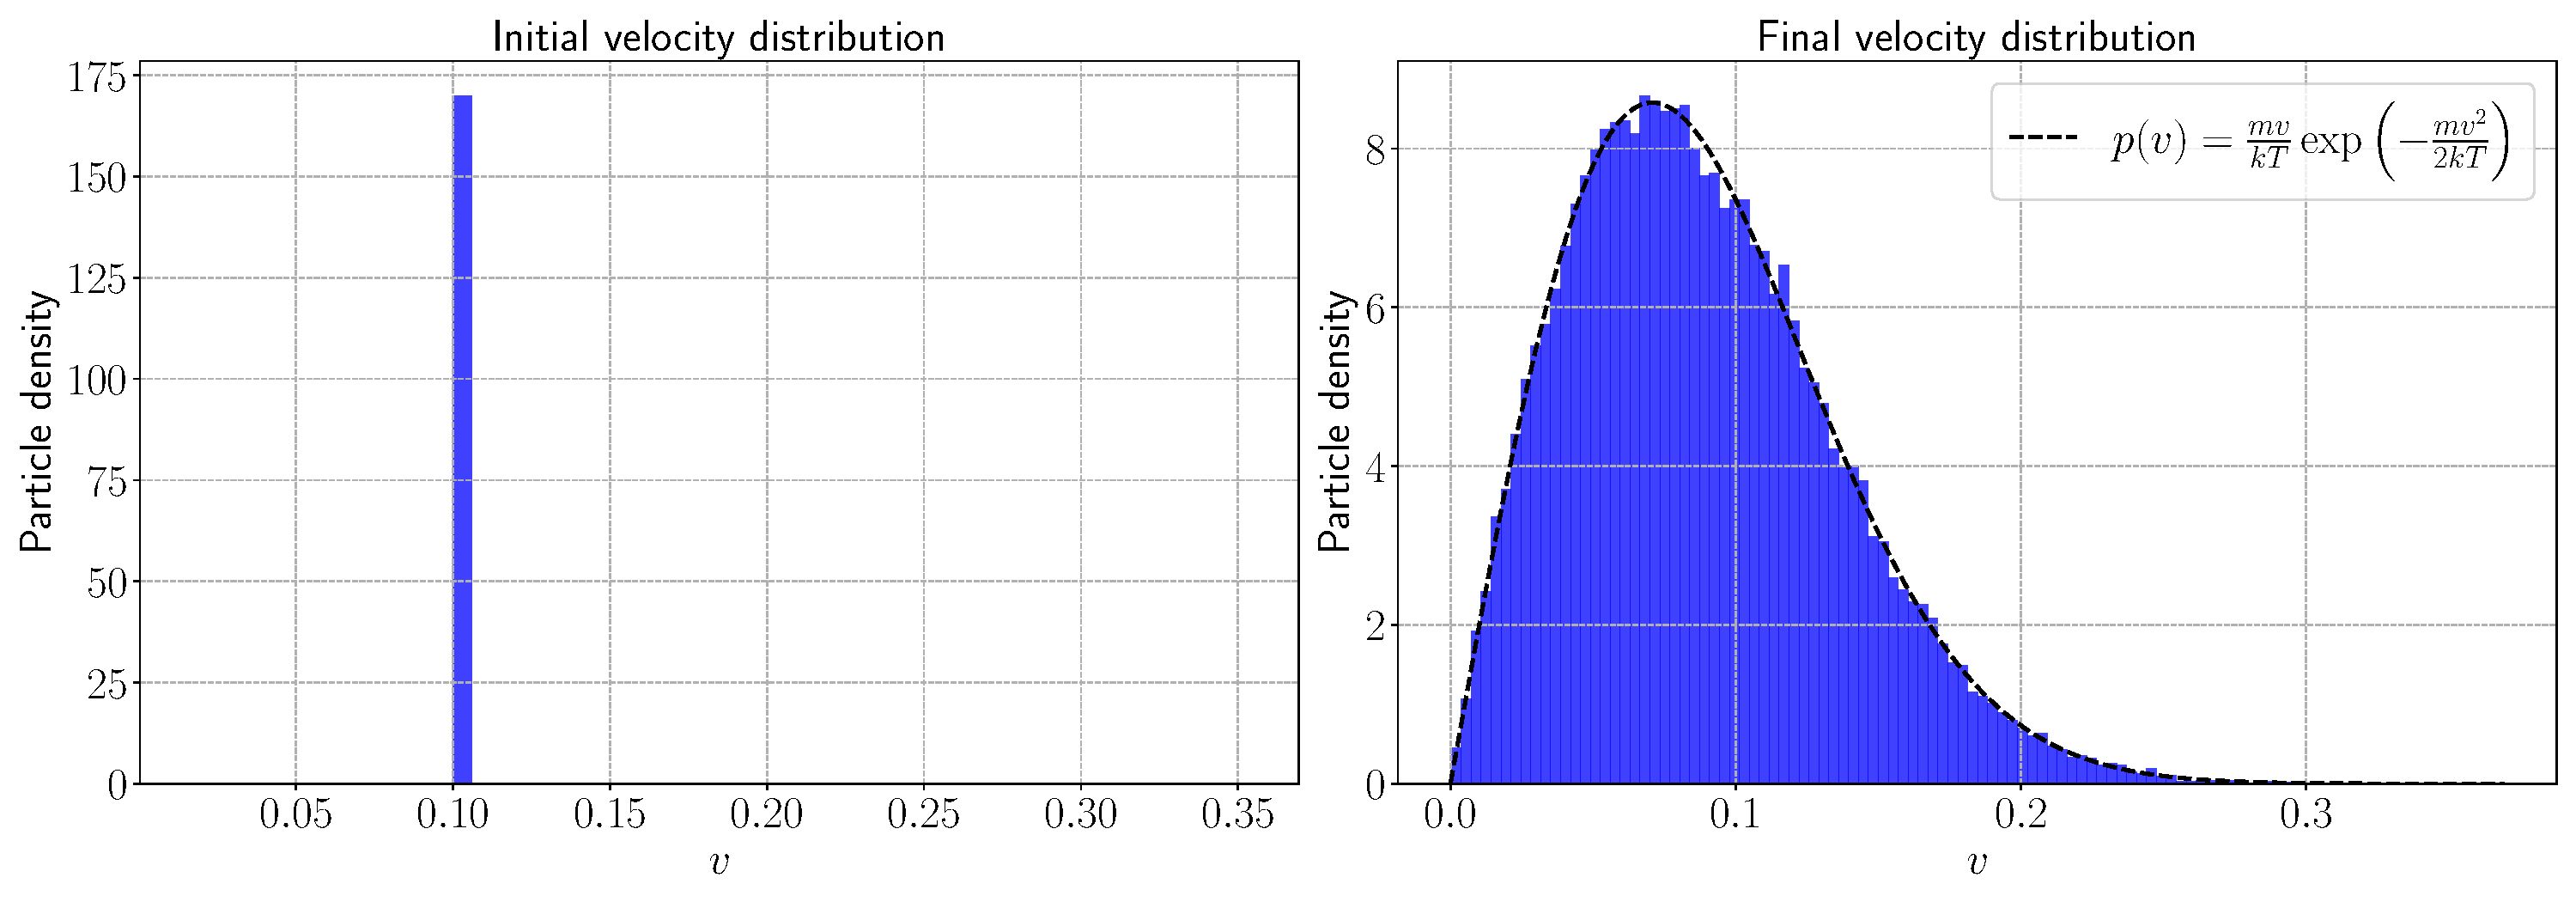
\includegraphics[width=\textwidth]{../fig/distribution}
	\caption{Distribution of velocities in a gas of $50000$ particles.}
	\label{fig:dist_1}
\end{figure}

To make the comparison more quantitative, we plot the difference between the Gaussian kernel density estimation of the final distribution and the Maxwell distribution. 

\begin{figure}[htb]
	\centering
	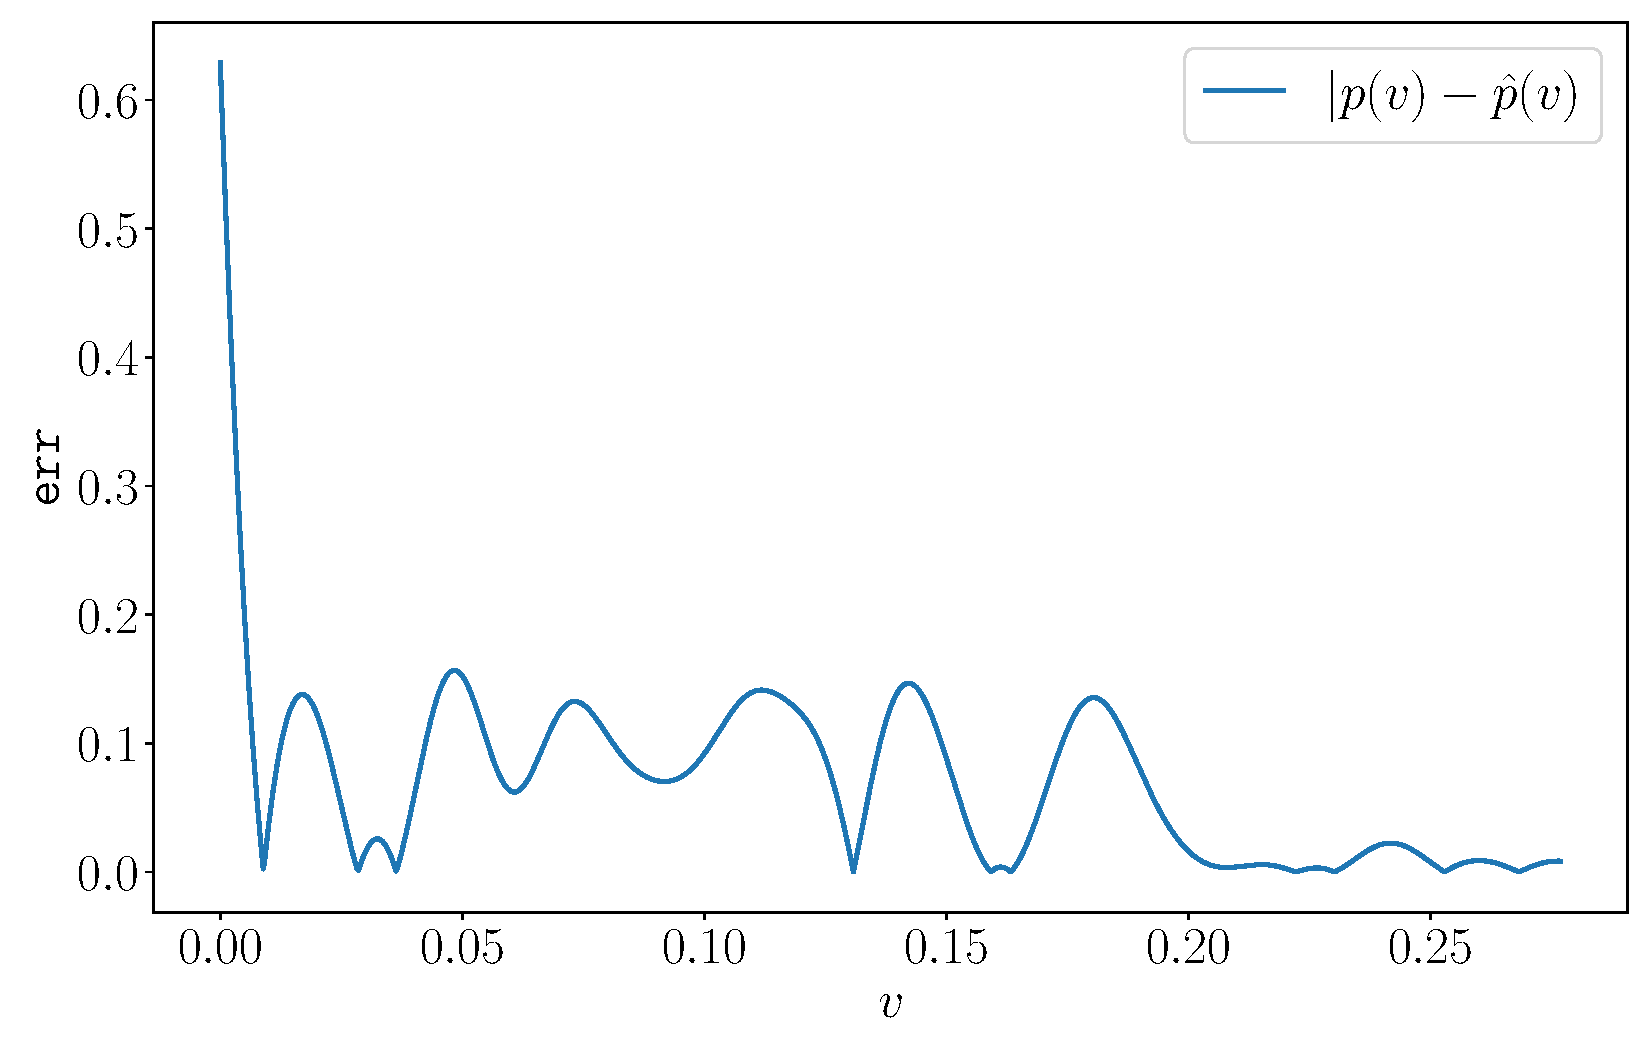
\includegraphics[width=0.8\textwidth]{../fig/kde_diff}
	\caption{Deviation between Gaussian kernel density estimation of the velocity distribution, $\hat{p}(v)$ and the Maxwell-distribution $p(v)$.}
	\label{fig:dist_2}
\end{figure}

\section{Mixture of two gases}\label{sec:mix1}

We repeat the exact same procedure as in section \ref{sec:eq}, except that we make half of the masses $4$ times as big as the rest. The velocity distributions after equilibrium is reached is plotted in \ref{fig:dist_3}.

\begin{figure}[htb]
	\centering
	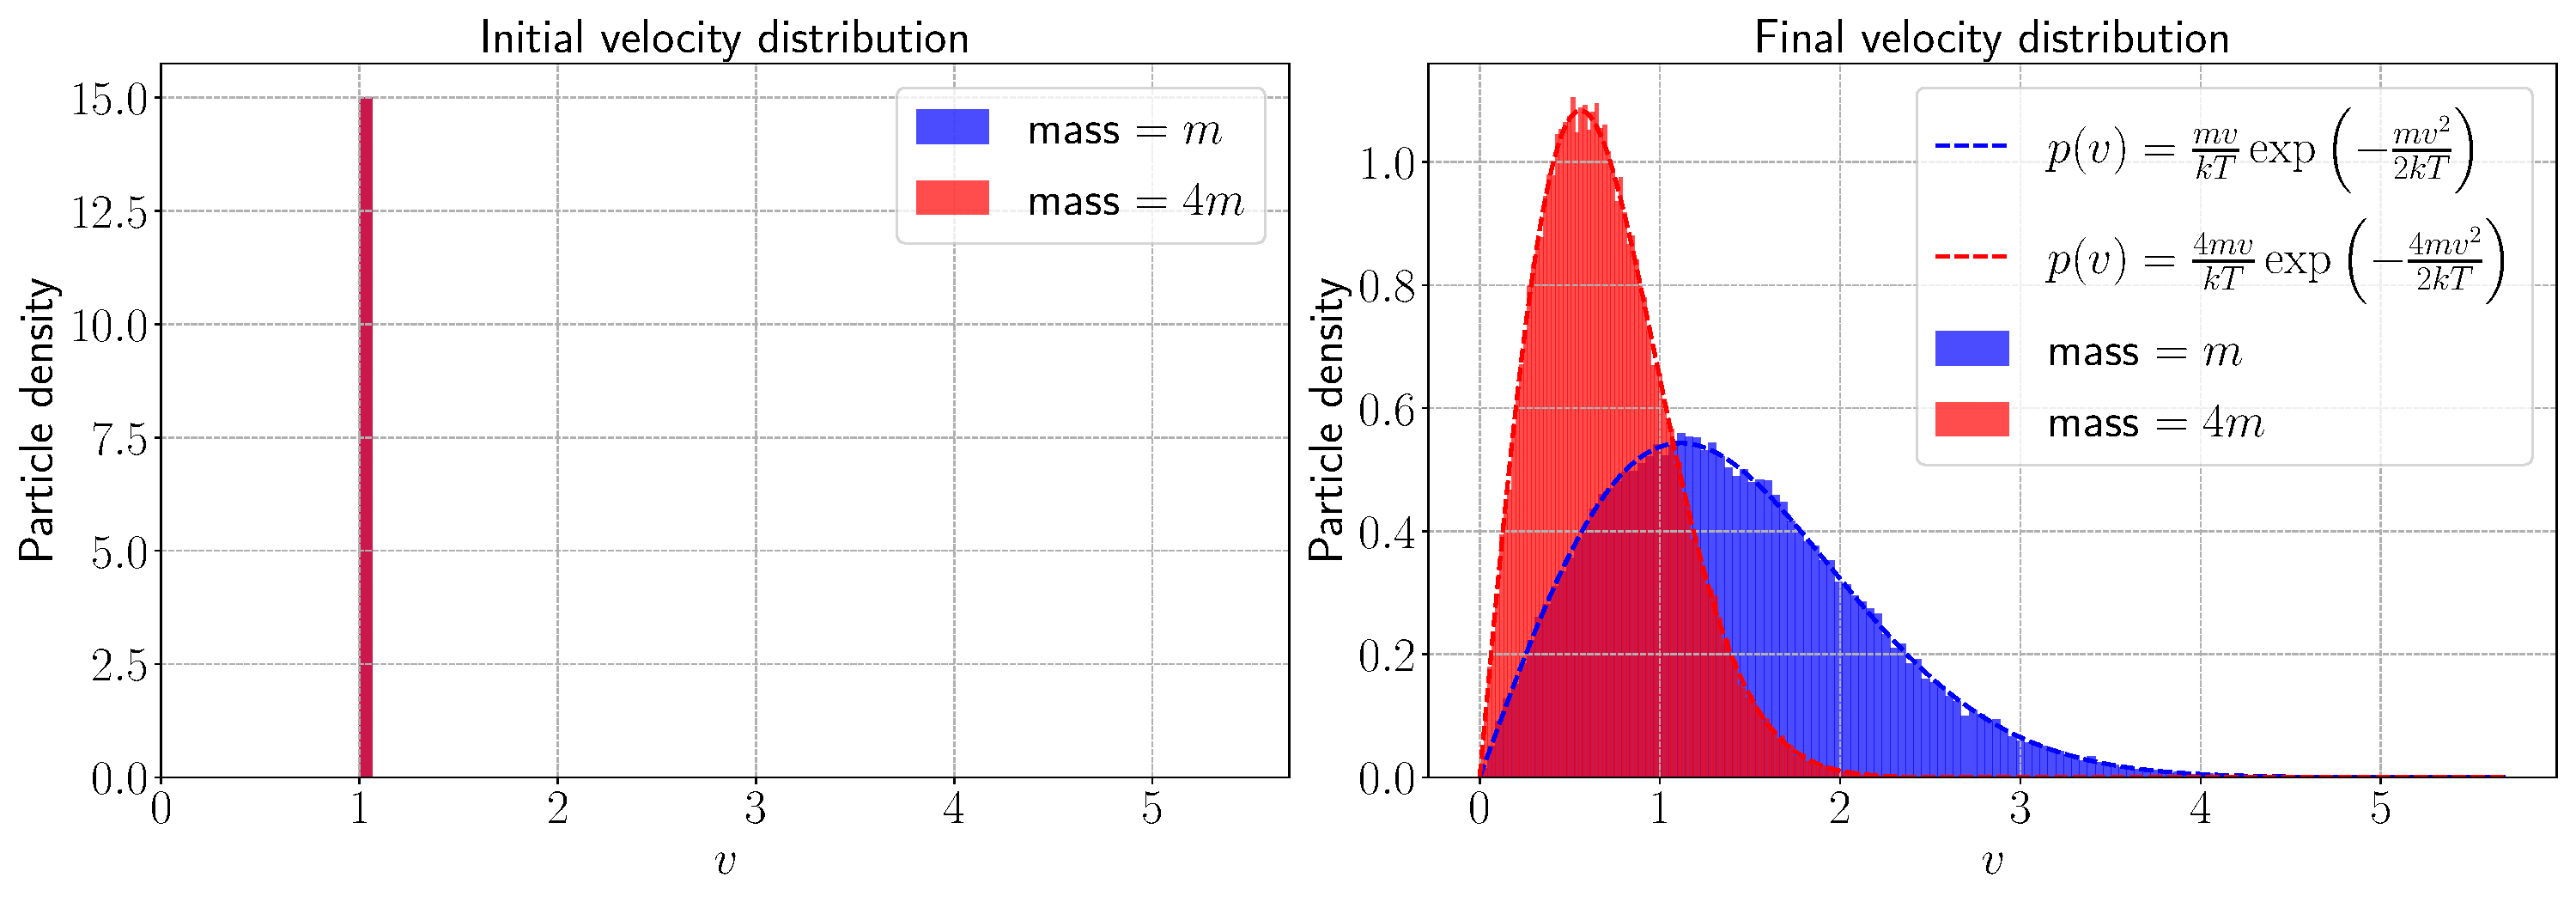
\includegraphics[width=\textwidth]{../fig/distribution_2}
	\caption{Distribution of velocities in a gas of $50000$ particles. The red distributions correspond to the heavy particles, while the blue correspond to the lighter particles.}
	\label{fig:dist_3}
\end{figure}

The average speed and kinetic energy is shown in table \ref{tab:averages}. These results suggests that although the masses are different, the mixture of the gases eventually reach equilibrium.  

\begin{table}[htb]
	\centering 
	\caption{Average speed and kinetic energy for the light and heavy particles}
	\begin{tabular}{ccc}
		\hline
		\textbf{Mass }& \textbf{Average speed} & \textbf{Average kinetic energy} \\
		\hline 
		$m$   & 0.1400 & 0.1259 \\
		$4m$  & 0.0699 & 0.1241 \\
		\hline 
	\end{tabular}
	\label{tab:averages}
\end{table}


\section{Mixing in the presence of energy dissipation}\label{sec:mix2}

To investigate, at least visually, whether the gas mixture reaches equilibrium we plot the time evolution of the averages of the energy of each species. In addition, we include two similar cases with the restitution parameter $\xi$ set to $0.9$ and $0.8$. This is shown in figure \ref{fig:averages}. By the very definition of thermal equilibrium, e.g. the one given in \cite[p.~3]{huang}
\begin{displayquote}
	Thermodynamic equilibrium prevails when the thermodynamic state of
	the system does not change with time.
\end{displayquote}
it is clear that the system cannot reach equilibrium in the presence of energy dissipation. 

The plot in figure \ref{fig:averages} shows that the two different particle species reach equilibrium only in the case where the energy is conserved. Furthermore, it is seen that the heavy gas particles are always at higher temperature in the two latter cases. This is easily realised from the fact that the heavy particles start out at higher energy, as the speed of the molecules are the same initially. Even though energy will be transferred to the light particles as time evolves, the energy dissipation will eventually be larger than the gain, and so both types of particles will loose energy. As the total average is below the average of the heavy particles in the beginning, it will stay below for later times as well. 

\begin{figure}[htb]
	\centering
	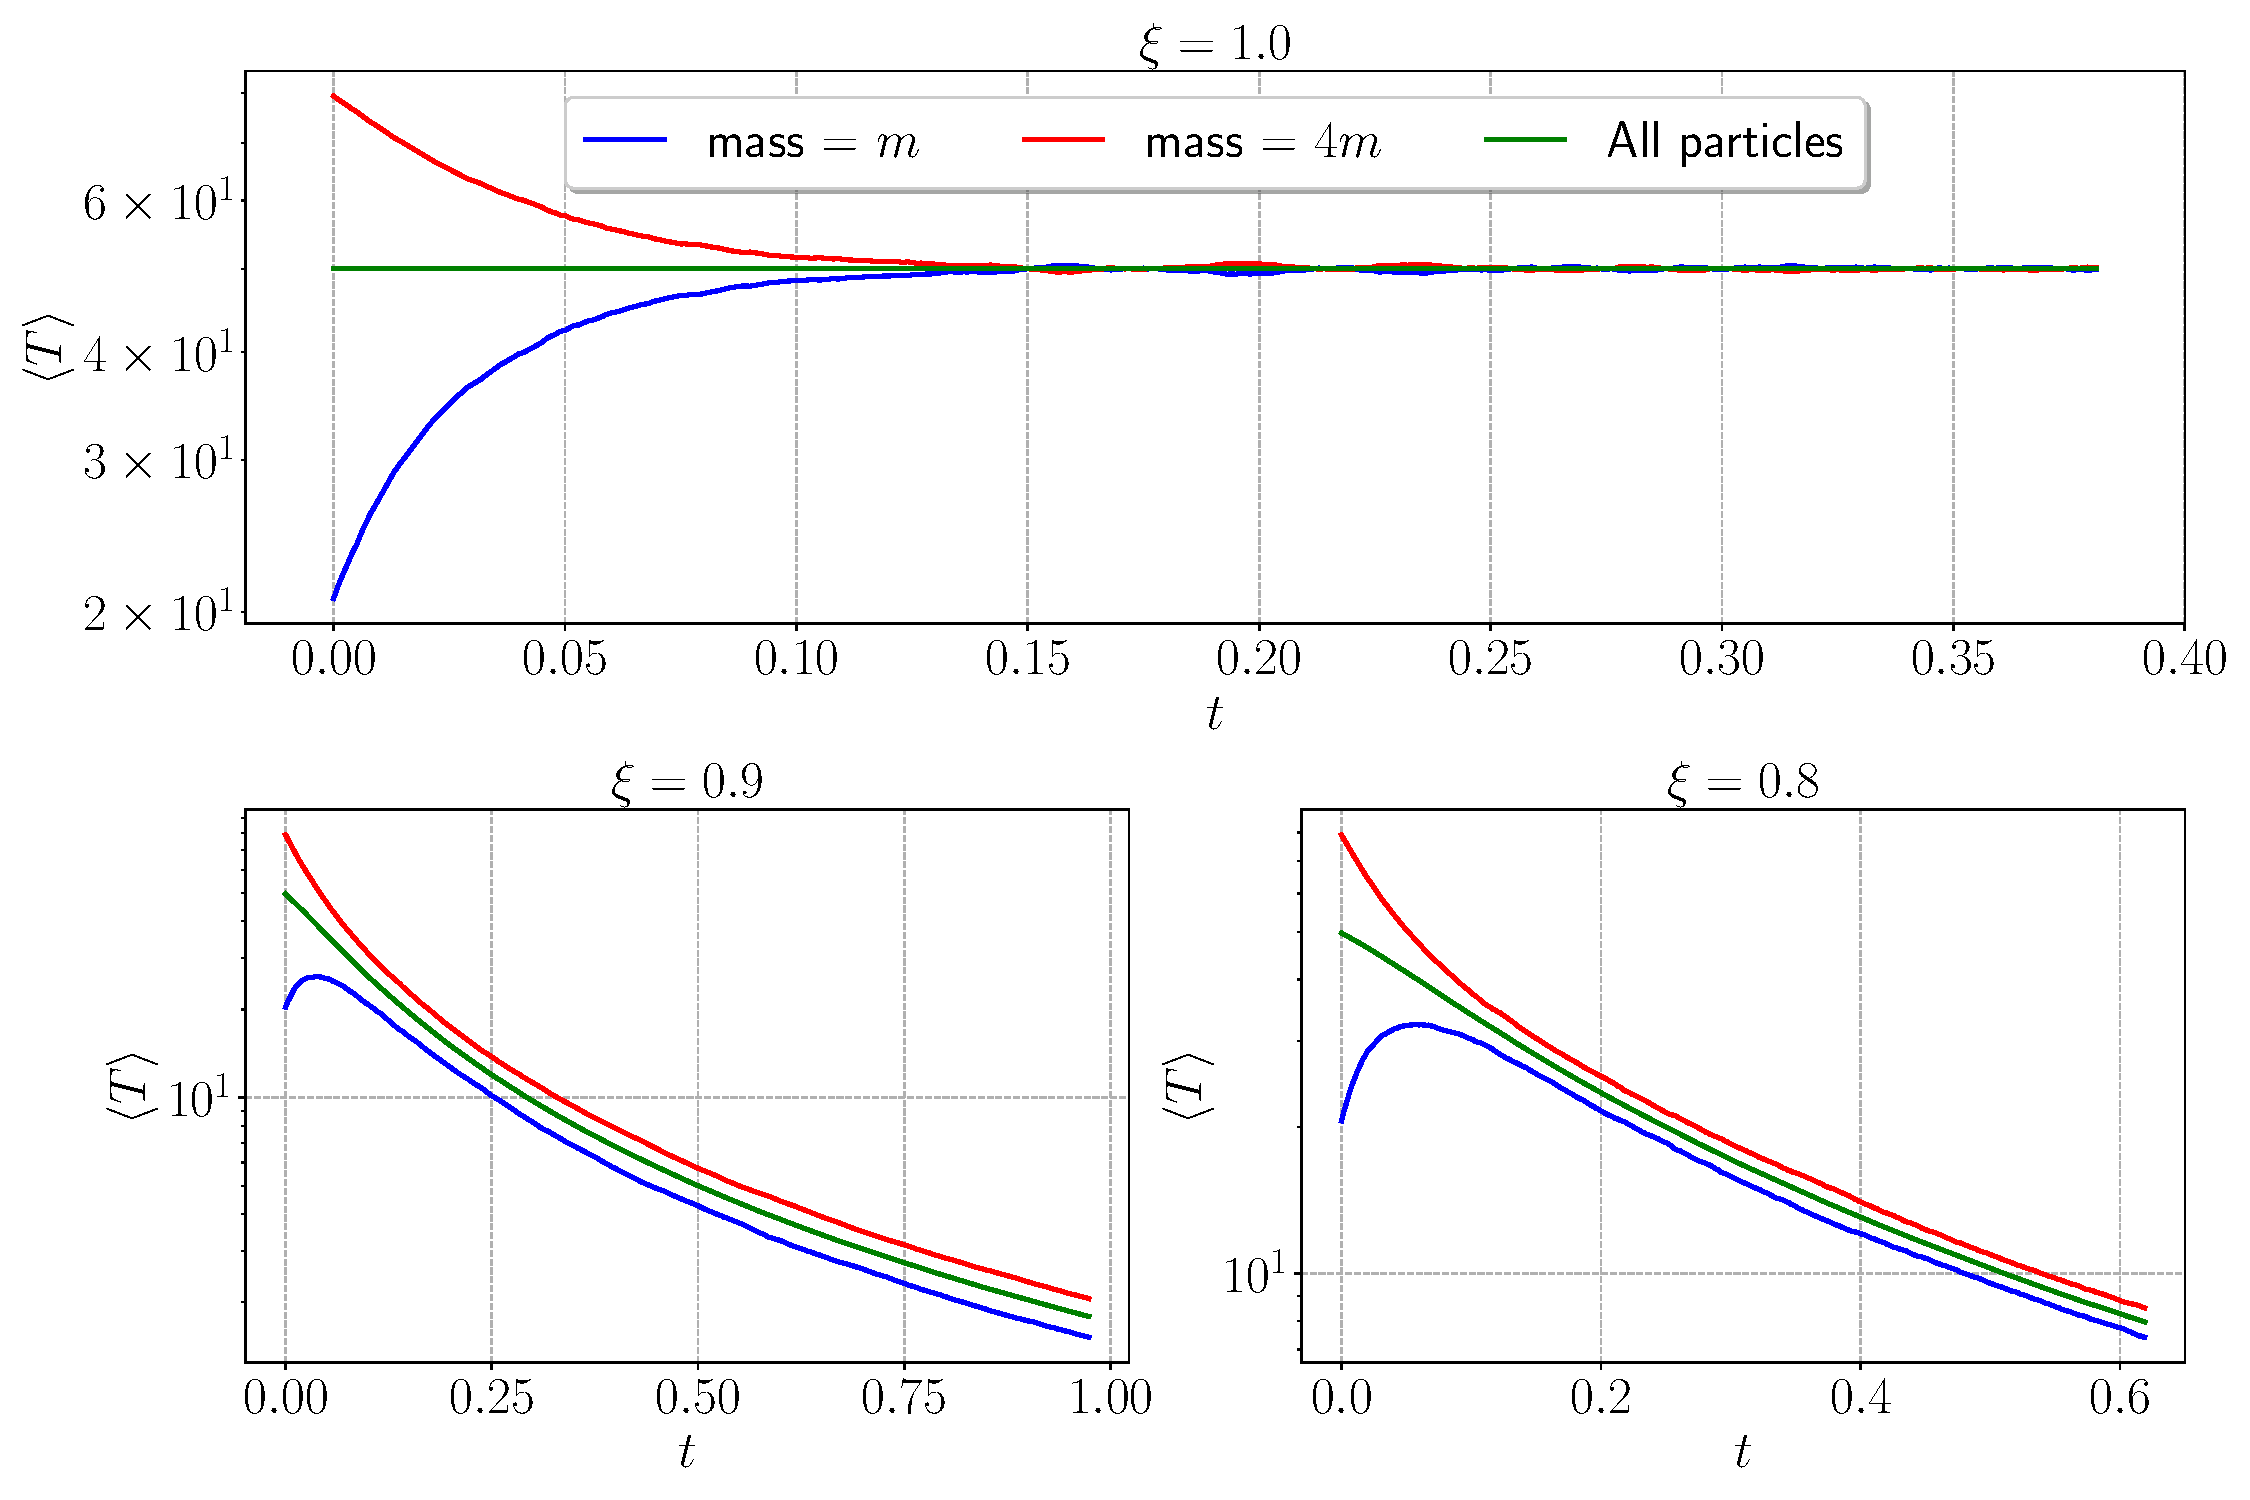
\includegraphics[width = \columnwidth]{../fig/energy_avg.pdf}
	\caption{Time evolution of energy averages for restitution parameter $\xi = 1.0,0.9,0.8$. The data comes from an ensemble of $8$ gases with $4000$ particles each.}
	\label{fig:averages}
\end{figure}

Although this fact is easily realised from elementary statistical mechanics, demonstrating it through these simulations is a good check that the correct physics is contained within the model made. 


\section{Crater formation from projectile impact}\label{sec:crater}

\subsubsection{Distributing the discs randomly in $[0,1]\times[0,0.5]$}

To distribute the particles randomly in the box defined by 
$$
\{(x,y)\in \RR : 0 < x < 1, 0 < y < 0.5\}
$$ 
I use the following scheme. 

To choose a suitable radius to have the particles fill up the available space with a packing fraction of $\rho \approx 1/2$ I solve for $r$ in 
$$
	N \pi r^2 = A(r) \rho = \frac{1}{2} A(r),  
$$
where, in order to avoid having particles outside the box, the area depends on $r$. If we clear a border of $r$ on the boundary of the region facing the walls, we get $r$ from solving

\begin{equation}\label{eq:r}
	N \pi r^2 = \frac{1}{2} \left(1- \frac{1}{2}r\right) \left(1-2r\right) \quad \Rightarrow \quad r = \frac{-1 + \sqrt{N\pi}}{2(N\pi - 1)}.
\end{equation}

To avoid having overlapping particles, I do the following

\begin{algorithm}[H]
	Choose number of particles $N$\;
	Find $r$ corresponding to $N$ from \eqref{eq:r}\;
	$\mathbf{x} \gets [(0,0),\dots,(0,0)]$\;
	Sample $x_i \sim \mathcal{U}_{[r,1-r]}$ and $y_i \sim \mathcal{U}_{[r,0.5]})$\;
	$\mathbf{x}_0 \gets (x_i,y_i)$\;
	\For{$i = 2\dots N$ }{
		Sample $x_i \sim \mathcal{U}_{[r,1-r]}$ and $y_i \sim \mathcal{U}_{[r,0.5]})$\;
		$\mathbf{x}_i \gets (x_i,y_i)$\;
	\While{Particle $i$ does not overlap with particle $1,\dots,i-1$}{
		Sample $x_i \sim \mathcal{U}_{[r,1-r]}$ and $y_i \sim \mathcal{U}_{[r,0.5]})$\;
		$\mathbf{x}_i \gets (x_i,y_i)$\;
	}}
	\caption{Non-overlapping random placement of discs in rectangular region.}
\end{algorithm}  

\subsubsection{Illustration of crater formation}

The plots in figures \ref{fig:crater_1} and \ref{fig:crater_2} shows the crater formed when the mass of the projectile is $5$ and $25$ times the mass of the particles in the bed, respectively. The darker the colour of the particles, the more collisions they have been involved in. Define the \textit{size of the crater}, $\mathcal{S}$, as the number of affected particles by the impact. That is, the number of particles moved during the impact. In the illustrations in figures \ref{fig:crater_1} and \ref{fig:crater_2} the size is the number of non-yellow particles. 

\begin{figure}
	\centering
\begin{minipage}{0.48\columnwidth}
		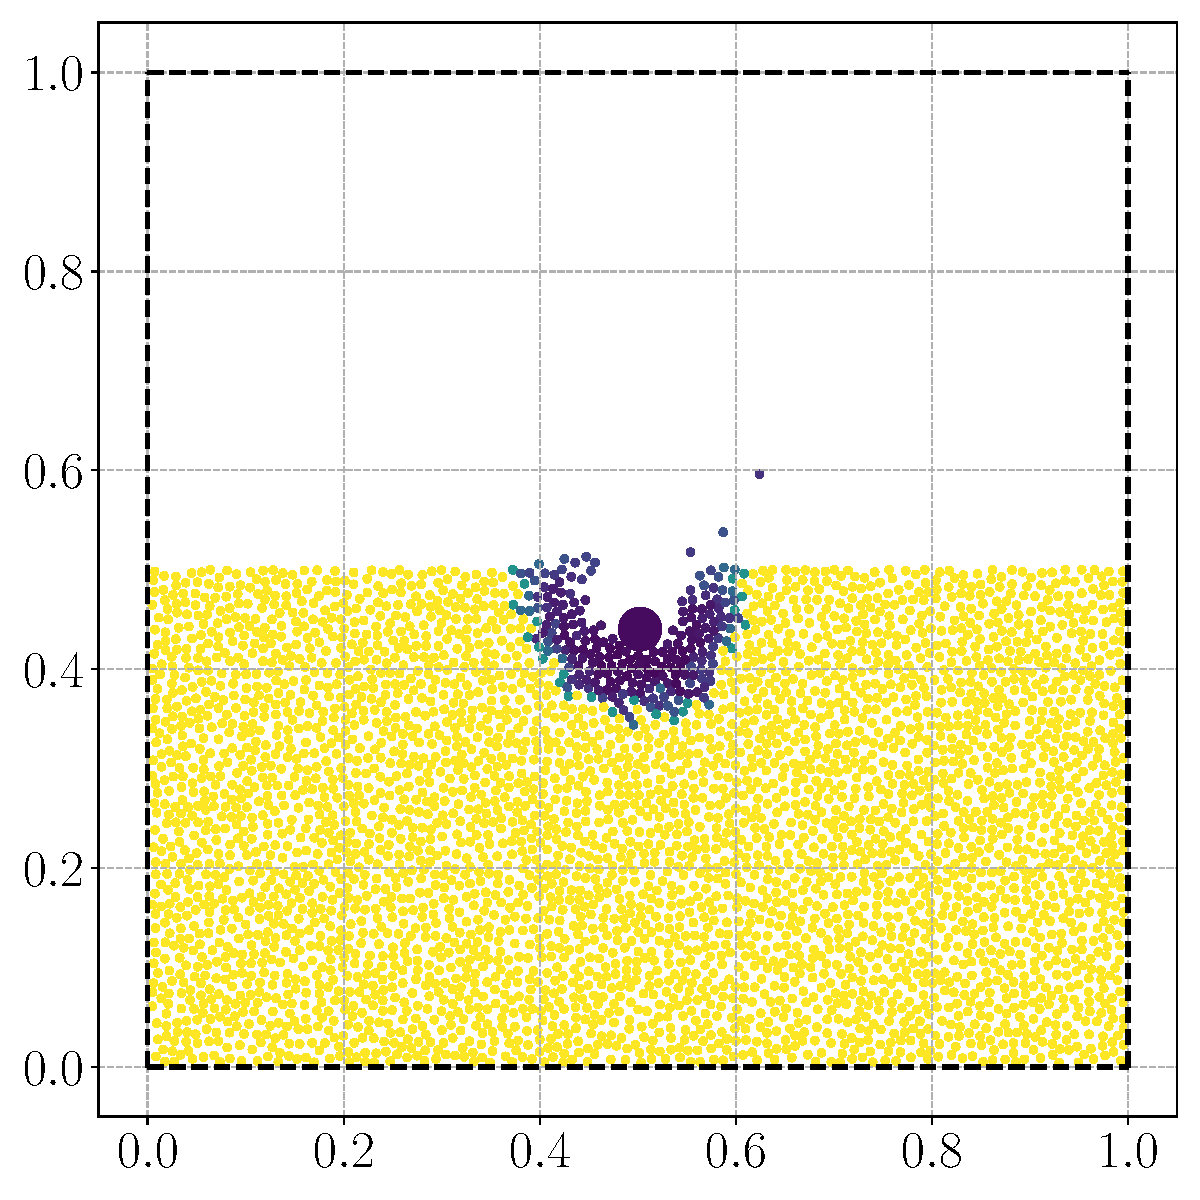
\includegraphics[width=\linewidth]{../fig/crater_1}
		\captionof{figure}{Example of crater formation using a projectile mass $5$ times the mass of the remaining particles.}
		\label{fig:crater_1}
\end{minipage}
\hfill
\begin{minipage}{0.48\columnwidth}
		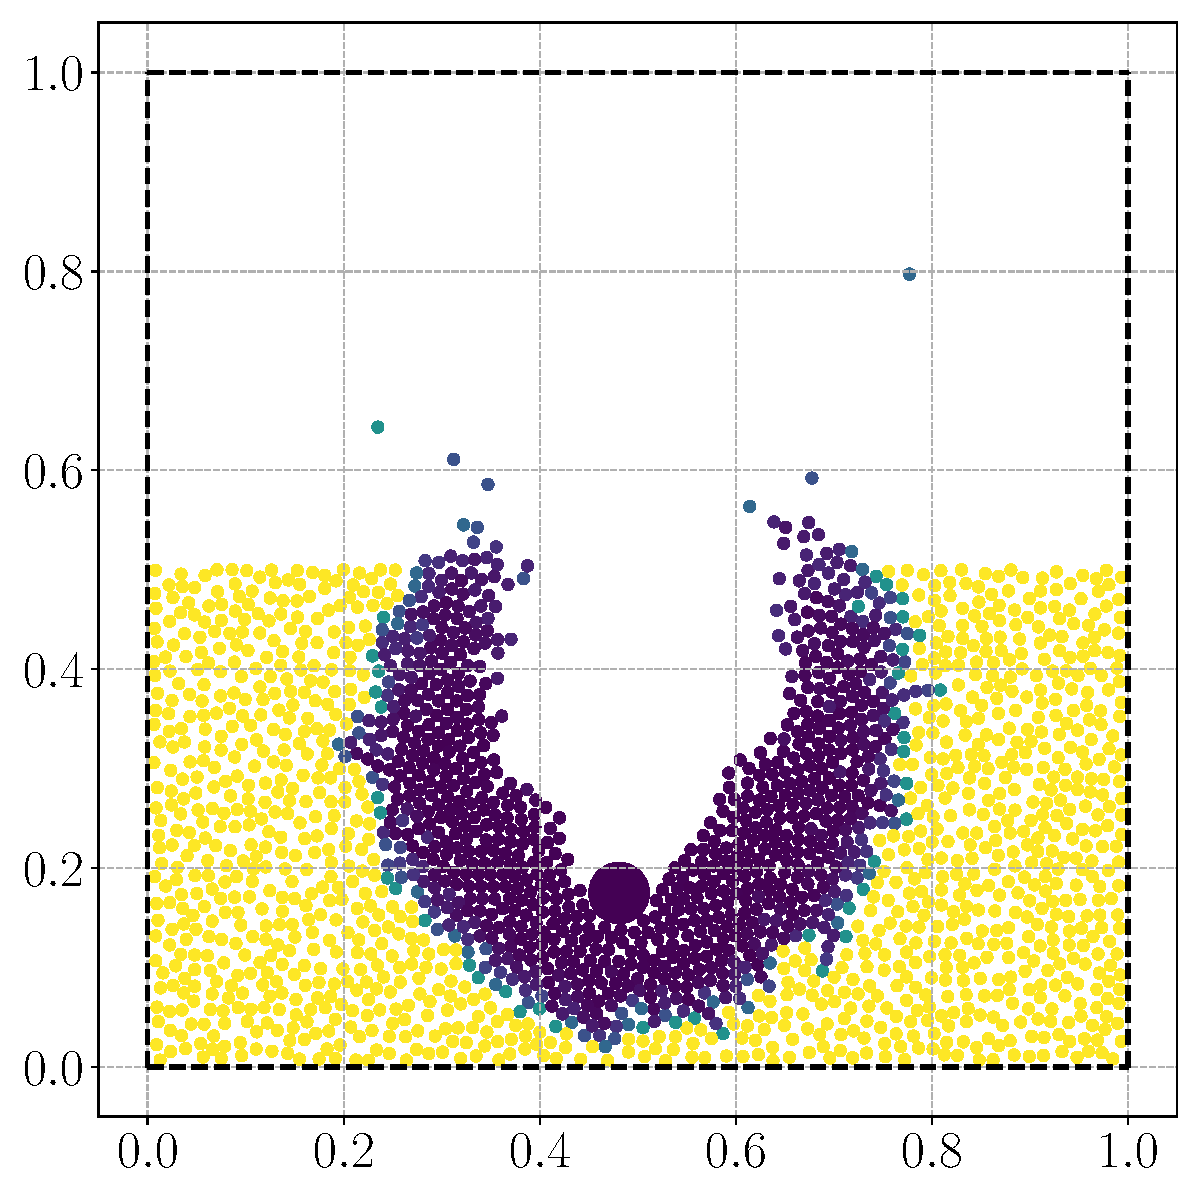
\includegraphics[width=\linewidth]{../fig/crater_2}
		\captionof{figure}{Example of crater formation using a projectile mass $25$ times the mass of the remaining particles.}
		\label{fig:crater_2}
\end{minipage}
\end{figure}
\subsubsection{Scanning over the projectile mass}

By simulating crater formation with projectile masses running from $1$ to $25$ times the mass of the remaining particles, the size of the crater is as shown in figure \ref{fig:mass_size}. The size of the crater $\mathcal{S}$ is simply the number of particles involved in the crater formation. The plot clearly shows that a larger projectile mass gives rise to a larger crater, as one intuitively would expect. 

\begin{figure}
	\centering
	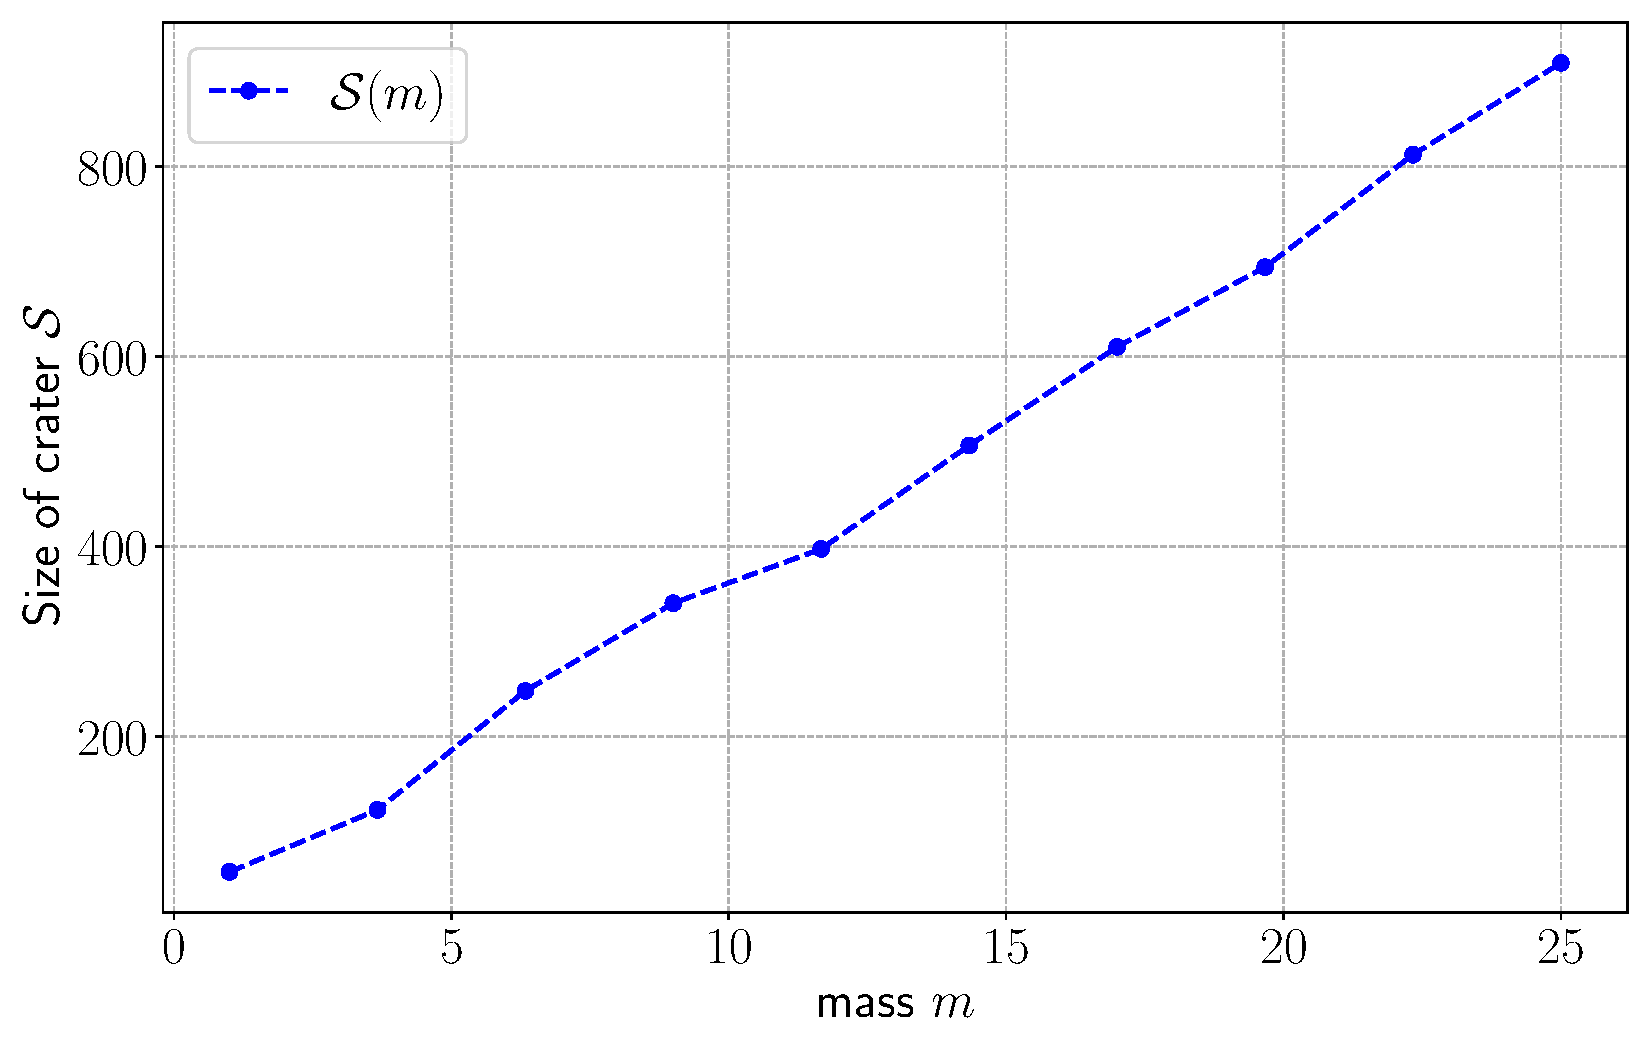
\includegraphics[width=\columnwidth]{../fig/mass_size}
	\caption{Size of crater as a function of projectile mass. The values are calculated from the mean of simulating projectile impact on $8$ ensembles of a bed of $2000$ particles.}
	\label{fig:mass_size}
\end{figure}

\newpage
%\part{Conclusion}
\part{Conclusion}

We have used a event-driven procedure to simulate a $2$-dimensional gas of colliding discs. As predicted by classical statistical mechanics, the distribution of speeds of the particles in this gas follows the Maxwell-Boltzmann distribution in equilibrium. In the presence of energy dissipation, a system consisting of heavy and light gas particles is demonstrated to \textit{not} reach equilibrium. These demonstrations indicates that this simulation approach agrees with the more orthodox method of integrating the equations of motion. This fact is quite remarkable as the method used here only relies on the assumption that the particles undergo linear motion with constant velocity between the collisions, with no mention of any Hamiltonian nor Newtonian equation of motion.
%Add a conclusion here if necessary


\bibliographystyle{alpha}
\bibliography{references}

\end{document}